\documentclass[12pt,journal]{IEEEtran}

\usepackage[utf8]{inputenc}
\usepackage{pgfplots}
\usepackage{caption}
\usepackage{mathtools}

\begin{document}

    \title{Lineal regression with two variables}
    \author{Alejandro Salgado G}
    \maketitle

    This problem consists in predicting differents ouputs based on some examples
    that the algorithm in going to receive. \\



    \begin{figure}[h]

        \centering
        \captionsetup{justification=centering}

        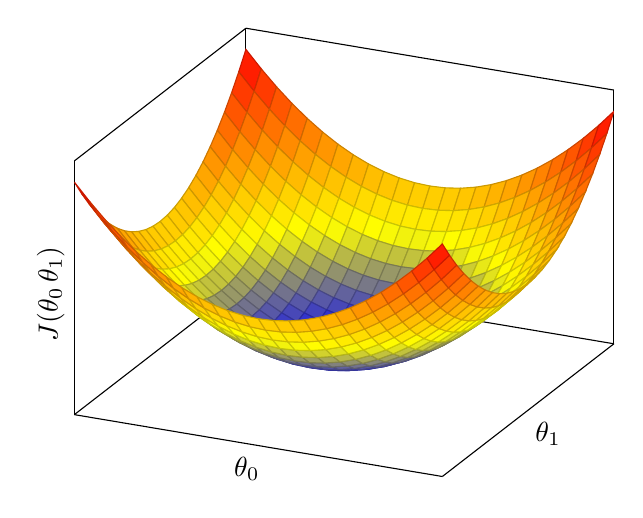
\begin{tikzpicture}
            \begin{axis}[
                            xlabel=$\theta_0$,
                            ylabel=$\theta_1$,
                            zlabel=$J(\theta_0 \, \theta_1)$,
                            xtick=\empty,
                            ytick=\empty,
                            ztick=\empty
                        ]
                \addplot3[surf]{x^2+y^2};
            \end{axis}
        \end{tikzpicture}

        \caption{Cost function}
    \end{figure}

\end{document}
